\chapter{Control analysis of the DNA repair rate}
\label{chap:robustRepair}

In the previous chapter we introduced the incorporation of EdU upon UV-irradiation as a quantitative readout for the DNA repair synthesis kinetic (cf.\ Figure \ref{fig:EdU_measurement}). We could show that despite the pathway's complexity, DNA repair follows a mono-exponential kinetic of first order. Moreover, the repair of single lesions is distributed over a broad time with a half-time of $\sim$1.2 h. Notably, measurements on the single cell level revealed also that the half-time and hence the rate of repair is highly variable (cf.\ Figure \ref{fig:DNArepairKinetic}B-E). So far, not only is the origin of this heterogeneity unknown, but also how the cell faces this highly variable environment.\\  
In this chapter we will apply the previously introduced kinetic NER model and explore the nature of the repair rate variability. By simulating the effect of NER factor variation on the repair rate, we find that the repair rate control is distributed among all NER factors. Exploiting the natural variability of repair proteins we can experimentally corroborate the computationally-derived finding for the NER factors XPC, TFIIH, XPA, XPF and RPA. Apart from the variability in protein expression, the model identifies the initial amount of inflicted DNA damage as major contribution determining the repair rate distribution. Both sources combined appears to be sufficient to explain the overall rate variability.\\     

The work reported in this chapter has been done in close collaboration with Paul Verbruggen who planned and conducted the experiments.

\section{Kinetic NER model predicts collective rate control}
\label{sec:repairControl}

The narrow confidence bounds derived by PLE analysis identified parameters in reasonable biological ranges (cf.\ Section \ref{sec:identifiabilityAnalysis}) allowed us to use the model for quantitative predictions. On the basis of the simplified model result, indicating that the fast and random enzyme exchange defines the slow first-order rate kinetics (cf.\ Section \ref{sec:toyModel}), we wanted to test whether this concept of multi-protein rate control also applies on the realistic NER model. To determine the response of a system to changes in the environment, one can calculate the response coefficients $\tilde{R}_i$ \cite{Hofmeyr1991,Fell1992}. Accordingly, we can quantify the relative change in the repair rate $\nu$ as a function of the relative change in the protein concentration $C_i$ ($i$ = XPC, TFIIH,...).

\begin{equation}
\tilde{R}_i = \frac{\partial \, \text{ln} \, \nu}{\partial \, \text{ln} \, C_i}.
\label{eqn:responseCoefficients}
\end{equation}

The inverse of $\nu$ is the characteristic time $\tau_R$ that represents the time duration for the repair reaction $R$. Hence, Eqn.\ \ref{eqn:responseCoefficients} can be rewritten as

\begin{equation}
\tilde{R}_i = \frac{C_i}{\tau_R^{-1}} \frac{\partial  \, \tau_R^{-1}}{\partial \,  C_i}.
\label{eqn:rC_characteristicTime}   
\end{equation}

$\tau_R$, in turn, can be directly approximated from the distribution of repaired DNA states $y^R_\pi(t)$, which include the modelled DNA intermediates for resynthesised and rechromatinised DNA. By taking the ratio between the first ($\mu^{(1)}$) and the zeroth ($\mu^{(0)}$) central moment of the distribution we derive the reaction-specific mean time 

\begin{equation}
\tau_{R} = \frac{\mu{(1)}}{\mu^{(0)}}, 
\label{eqn:meanreactiontime}   
\end{equation}

with

\begin{equation}
\mu^{(m)} = \int t^m \, y^R_\pi(t)\, dt.
\label{eqn:moments}   
\end{equation}


To ensure the convergence of the integral we subtract all repair synthesis states (IV + V) from the initial amount of damages $y^{\text{I}}_{00} = $ 3.33 \textmu M at t = 0.

\begin{equation}	
\tau_{\text{syn}}=\frac{\int (y^I_{00}(0)-( \sum_ \pi  y_\pi^{IV}(t)+\sum_ \pi  y_\pi^{V}(t))\; dt)\cdot t\; dt}{\int y^I_{00}(0)-( \sum_ \pi  y_\pi^{IV}(t)+\sum_ \pi  y_\pi^{V}(t))\; dt}
\end{equation}

Using $\tau_{\text{syn}}$ in Eqn.\ \ref{eqn:rC_characteristicTime} we derive the response coefficients for the repair synthesis rate, which are uniformly small with $\sim$0.3 and below (cf.\ Figure \ref{fig:controlCoefficients}). This result implies that there is no single repair protein whose effect on the repair speed could be interpreted as rate-limiting. A similar result is obtained for the rate of re-synthesis response coefficients (cf.\ Figure \ref{fig:cc_rateOfincision}), with the characteristic time

\begin{equation}
\tau_{\text{inc}}=\frac{\int^\infty_0 \,t \,\sum_{x=I}^{\text{III}} \sum_ \pi  y_\pi^x(t)\,dt}{\int^\infty_0  \,\sum_{x=I}^{\text{III}} \sum_ \pi  y_\pi^x(t)\,dt}.
\end{equation}    



\begin{figure}[htbp]
	\begin{center}
		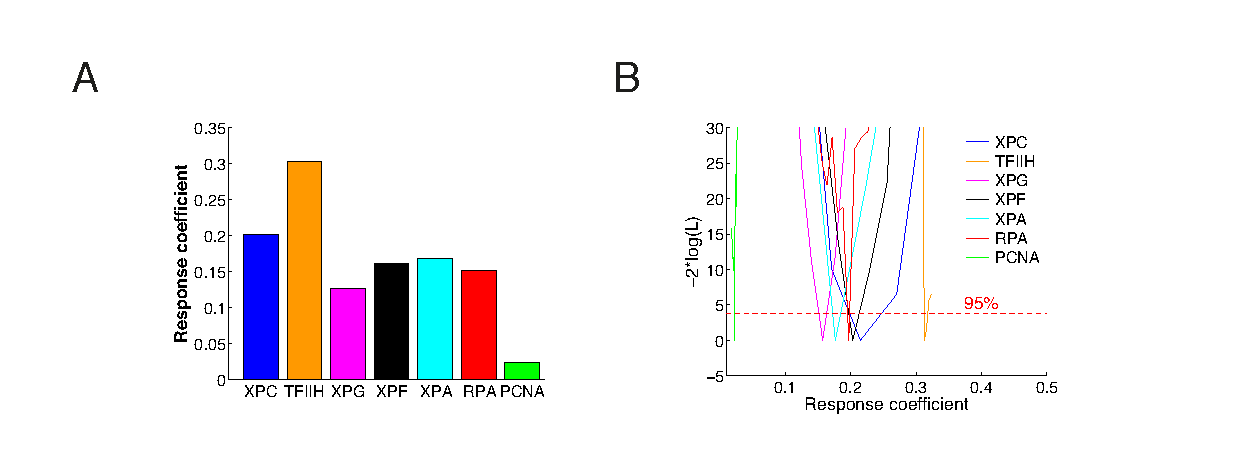
\includegraphics[width=1\textwidth]{Abbildungen/figure3_1.pdf}
		\caption{\textbf{Collective control of the repair rate.} A) Response coefficients for seven repair factors (XPC, TFIIH, XPG, XPA, XPF, RPA, PCNA) are small and uniformly distributed. B) Prediction profile likelihood indicate small prediction confidence bounds for each response coefficient. 95\% threshold is given by the $X^2$ distribution with one degree of freedom.}
		\label{fig:controlCoefficients}
	\end{center}
\end{figure}

\paragraph{Prediction profile likelihood}
To obtain realistic confidence bounds for the response coefficients we performed a prediction profile likelihood estimation \cite{Kreutz2012,Hinkley1979}. The predicted response coefficients $\tilde{R} = F(D_{\text{pred}},\theta)$ are considered as model outcomes $F$ for a predicted experimental design $D_{\text{pred}}= (z_{\text{pred}},t_{\text{pred}},u_{\text{pred}})$. $D_{\text{pred}}$ specifies a prediction observable $z_{\text{pred}}$ at time point $t_{\text{pred}}$ given the externally controlled stimulation $u_{\text{pred}}$. As defined in Eqn.\ \ref{eqn:observable} $z_{\text{pred}}(y(t),\theta)$ comprises a model simulation that can be mapped to experimentally observable quantities. Analogous to Eqn.\ \ref{eqn:PL}, the prediction profile likelihood 
\begin{equation}
PPL(\tilde{R}) = \max_{\theta^\ast \in \{\theta \lvert F(D_{\text{pred}},\theta)=\tilde{R}\}} L(z^\dag \lvert \theta^\ast,\tilde{r}) 
\end{equation}   

is obtained by maximization over the model parameters satisfying the constraint that the model response $F(D, \theta^\ast)$ after fitting is equal to the considered value $\tilde{r}$ for the prediction $\tilde{R}$ with respect to the measured data $z^\dag$. This procedure is repeated for continuous variations of $\tilde{R}$. The model response can then be expressed as 

\begin{equation}
\Delta X_{\theta_l}^2(\tilde{r}) = \min_{\{\theta, \tilde{r} \in \tilde{R}  \}} \left( X^2 (\theta,\tilde{r} )\right)
- \quad  \min_{\{\theta\}} \quad  \left( X^2 (\theta)\right),
\end{equation}

which describes the difference between the global $X^2$ minimum and the best fit with $r$ included into the objective function. Similar to Eqn.\ \ref{eqn:confidenceIntervals} we can determine prediction confidence bounds 

\begin{equation}
PCI_{1-a}(D_{\text{pred}},z^\dag) = \{\tilde{r}\textbar \Delta X_{\theta_l}^2(\tilde{r})\leq Q_{X^2}(1-a,1)\},
\label{eqn:confidenceIntervalsPPL}
\end{equation}

which include the set of predictions $\tilde{R} = F(D_{\text{pred}},\theta)$ for which -2log(PPL) is below the threshold given by the $X^2$-distribution. The PPLs were computed within the d2d-framework \cite{Raue2013} using the CVODE package \cite{Hindmarsh2005} for the numerical integration of the ODEs together with the sensitivity equations (cf.\ Section \ref{sec:maximumLL}).
By applying the PPL analysis for each response coefficient we find that all of them are identifiable indicating how well the model predictions are determined by the data (cf.\ Figure \ref{fig:controlCoefficients}B).\\ The moderate response predicted by the response coefficients also holds true for larger variations in the repair factor concentration (cf.\ Figure \ref{fig:R_largeProteinVariation}). The linear approximation (on which the response coefficients are based on) yields a reasonable description for about two-fold concentration decreases or increases (corresponding to a knock-down or overexpression experiment), while for very large decreases the repair rate drops eventually to zero (corresponding essentially to a gene knock-out). From this result we can conclude that the kinetic NER model predicts a collective NER factor control of the repair rate. Consequently, the repair pathway appears robust against natural fluctuations in repair protein expression.  


\begin{figure}[htbp]
	\begin{center}
		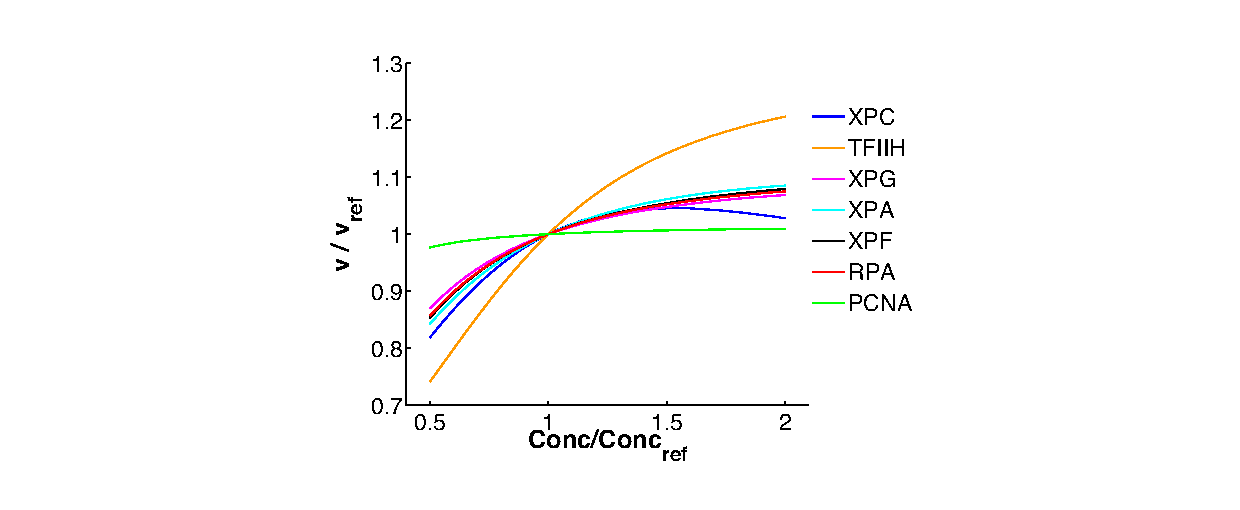
\includegraphics[width=1\textwidth]{Abbildungen/figure3_1_b.pdf}
		\caption{\textbf{Moderate repair rate response against natural NER factor expression variability.} Repair rate as a function of concentration changes in individual repair factors.}
		\label{fig:R_largeProteinVariation}
	\end{center}
\end{figure}

\section{Exploiting natural variability in protein expression to quantify rate control}
\label{natural_Variability_m}
To corroborate the model prediction of a distributed repair rate control (cf.\ Section \ref{sec:repairControl}), we developed an experimental set-up for the investigation of single repair factors and their quantitative influence on the repair rate. In particular, we asked whether there is a measurable response in the repair rate due to the natural occurring variability in protein expression. By capturing the integrated nuclear fluorescence intensity of antibody-stained repair proteins we derive the expression values for XPC, TFIIH, XPA, XPF and RPA. (cf.\ Figure \ref{fig:accuImage}B). For these five individually measured NER factors the expression variability was quantified by calculating the coefficient of variation (CV; standard deviation divided by the mean), which is on average $\sim$0.37 (cf.\ Figure \ref{fig:ProteinDist}A-E). Table \ref{tab:proteinVariability} gives the means and standard deviations from at least three biologically independent measurements of the expressed protein cell-to-cell variability.

\begin{table}[t!]
	\centering
	\begin{tabular}{cccccc}
		\hline
		\rule{0pt}{2ex}
		&\textbf{XPC} & \textbf{TFIIH} & \textbf{XPA} & \textbf{XPF} & \textbf{RPA}\\ \hline
		\rule{0pt}{3ex}
		\textbf{CV}: & 0.34 $\pm$ 0.05 & 0.33 $\pm$ 0.02 & 0.33 $\pm$ 0.03 & 0.4 $\pm$ 0.04 & 0.44\\ \hline
		
	\end{tabular}
	\caption{\textbf{Mean and standard deviation of the variability in nuclear XPC, TFIIH, XPA and XPF expression.} Distributions for nuclear protein expression were acquired in $\text{n}_\text{b}$(XPC) = 5, $\text{n}_\text{b}$(TFIIH, XPA,XPF) = 3 and $\text{n}_\text{b}$(RPA) = 2 independent biological replicates. Within each measurement between n=250 and n=572 with an average of n=477 cells were analysed.}\label{tab:proteinVariability}
\end{table}      

To distinguish whether the measured variability is due to differences in nuclear expression or rather superimposed by measurement noise, we co-analysed XPC-eGFP stably expressed in XP-C fibroblasts together with immunofluorescently labelled XPC in the same cell. Both quantities are strongly positively correlated (cf.\ Figure \ref{fig:ProteinDist}F) suggesting a large natural variability compared to much lower measurement noise. To quantitatively validate this observation, we performed a principal component analysis \cite{Pearson1901}. Thereby both quantities, XPC-eGFP and antibody-stained XPC intensities, are orthogonally transformed into a new coordinate system were the new transformed variables are linearly uncorrelated. These new variables are referred to as principal components. In a two-dimensional case the variances of both principal components define an error-ellipse as illustrated in Figure \ref{fig:ProteinDist}F. Calculating the CV from the smaller component we determined a relative measurement error for the antibody labelling method of $\sim$11\% showing that the technique is suitable for quantification of nuclear NER factor concentrations.       

\begin{figure}[htbp]
	\begin{center}
		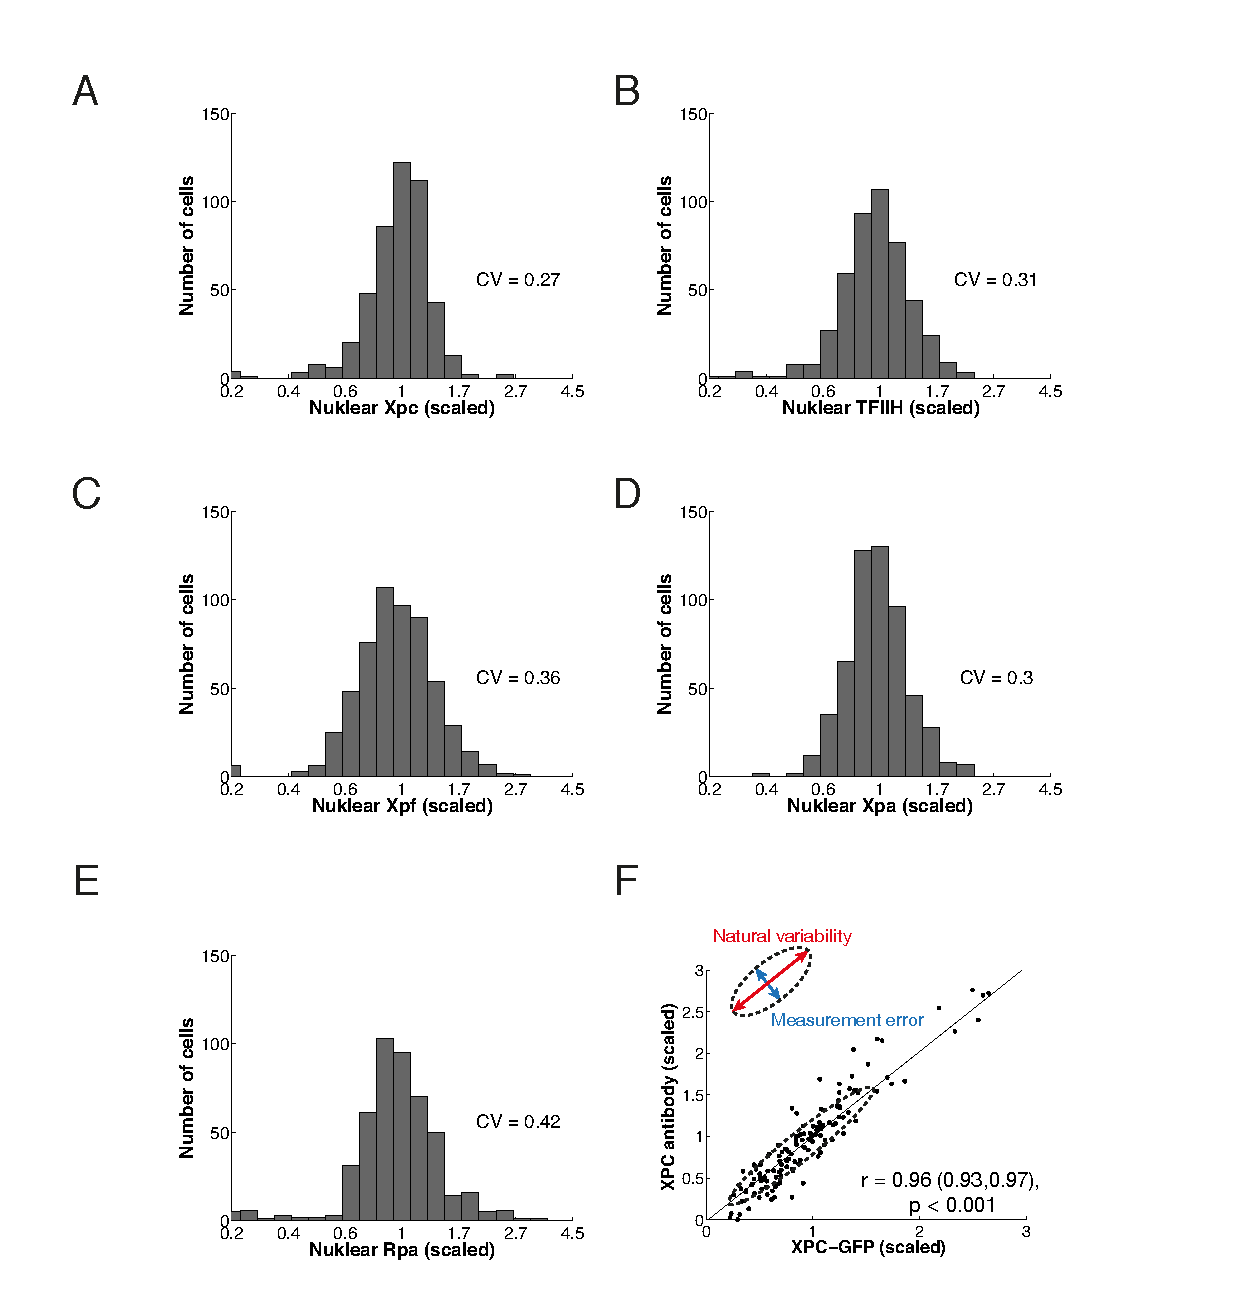
\includegraphics[width=1\textwidth]{Abbildungen/figure3_2.pdf}
		\caption{\textbf{Natural variability in nuclear NER factor expression is significantly larger than measurement error} A-E) Histograms of nuclear protein concentrations of the antibody stained NER factors XPC and TFIIH (n=470), XPF and XPA (n=565), RPA (n=487). F) Scatter plot of antibody stained XPC against XPC-eGFP stably expressed in XP-C XPC-eGFP cells. The dashed error-ellipse illustrates the proportion of natural variability and measurement noise.}
		\label{fig:ProteinDist}
	\end{center}
\end{figure}
%The same holds true for XPA \cite{Verbruggen2014}, TFIIH, XPF and RPA in narrow confidence bounds (cf.\ Appendix \textbf{tbm}).
Before exploring the direct relation between protein expression variability and the speed of repair we tested whether higher protein amounts in the nucleus correlate with the accumulation of NER factors in the locally damaged area. In correspondence to previous findings for XPG \cite{Luijsterburg2010} there is a significant positive correlation between the nuclear XPC-eGFP expression and its local accumulation at the DNA lesions (cf.\ Figure \ref{fig:Nuc_vs_DNAsynthesis}A) thirty minutes after UV irradiation. Consequently, we conclude that the DNA lesions are not saturated, and thus, a higher NER factor concentration could potentially accelerate the repair rate.\\
In fact, the nuclear protein concentrations for all five antibody-stained repair factors and the amount of incorporated EdU after one hour were weak, but still significantly correlated as indicated by the correlation coefficients and the corresponding small p-values (cf.\ Figure \ref{fig:Nuc_vs_DNAsynthesis}B-F). Remarkably, the dependency between protein concentration and EdU response, characterized by the slope of the regression line is very evenly distributed (cf.\ Figure \ref{fig:controlCoefficients}A). This agrees with the \textit{in silico} finding that the kinetic control of the measured repair factors is uniformly distributed and that the rate of repair synthesis is robust against natural variations in the repair protein expression.    

\begin{figure}[htbp]
	\begin{center}
		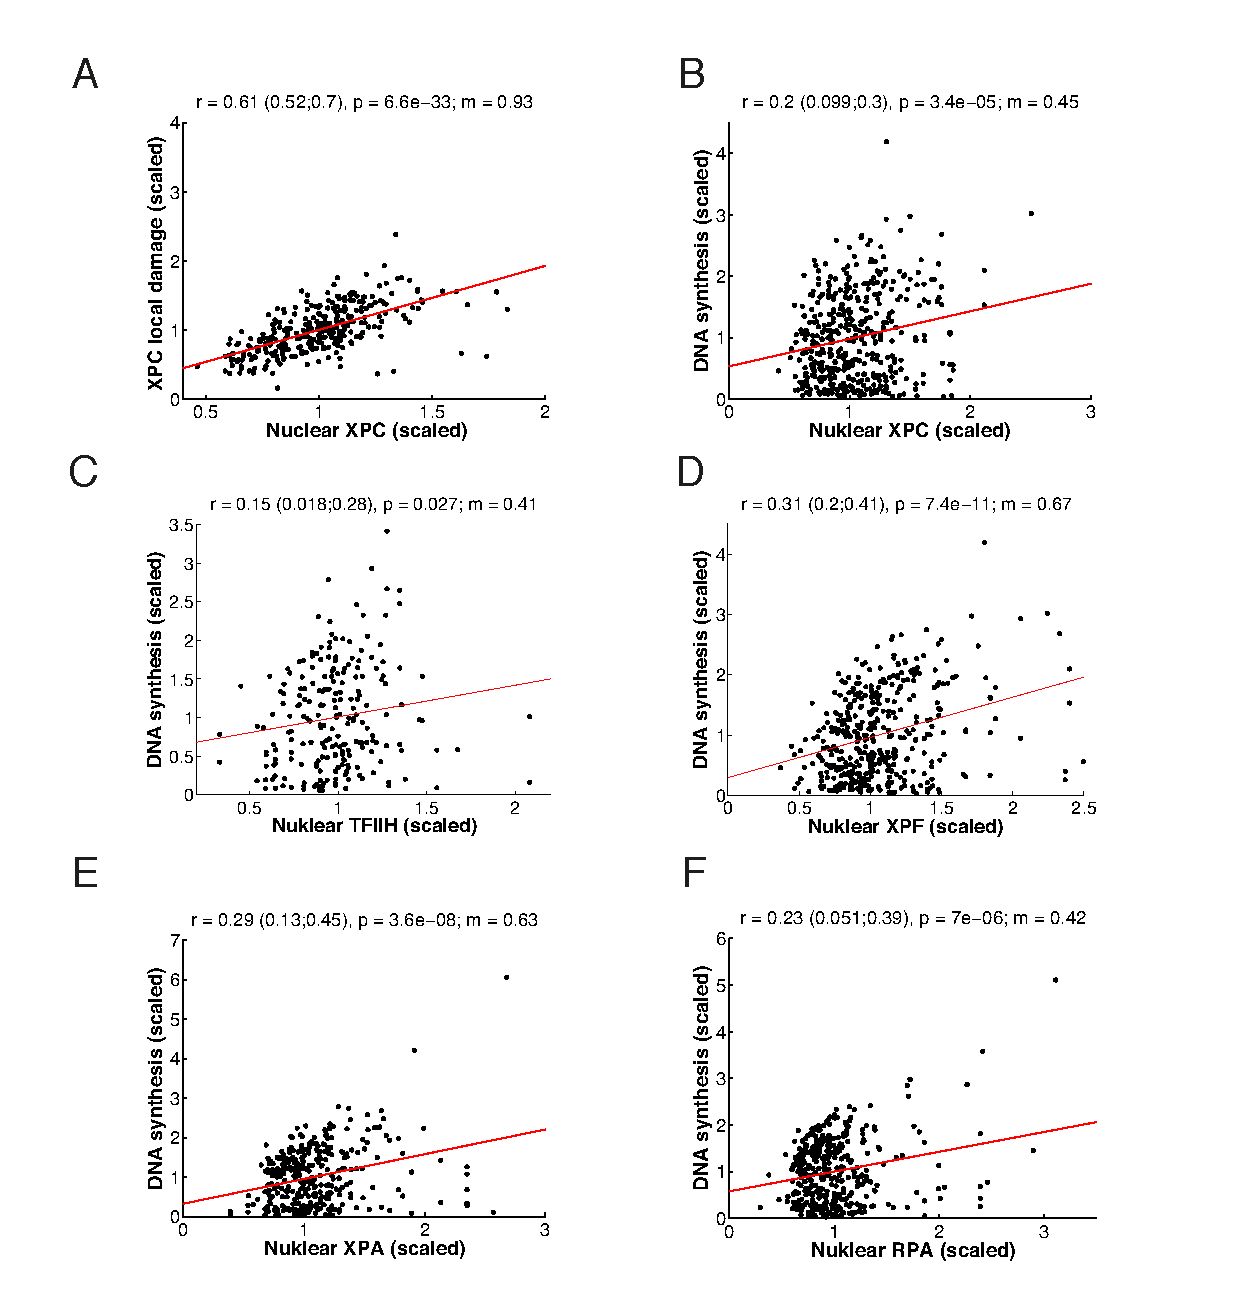
\includegraphics[width=1\textwidth]{Abbildungen/figure3_3.pdf}
		\caption{\textbf{Natural expression variability of the repair factors XPC, TFIIH, XPF, XPA and RPA has small effect on DNA repair synthesis.} A) Scatter plot of accumulated XPC in local damage against the nuclear XPC concentration (n=303) 60 minutes post irradiation. B-F) DNA synthesis correlated with the endogenous concentration of XPC (n=425), TFIIH (n=220), XPF (n=425), XPA (n=350) and RPA (n=383) 60 minutes post-irradiation. A-F) Red lines represent linear regression with correlation coefficient r, p-value and slope m. 95\% confidence bounds of all correlation coefficients r were estimated by non-parametric bootstrap and are given in brackets. }
		\label{fig:Nuc_vs_DNAsynthesis}
	\end{center}
\end{figure}

\paragraph{Correlation analysis}
The correlation analysis was performed in MATLAB (2012a, The Mathworks Inc., Natick, MA) using the inbuilt 'corrcoef' function, which also returns p-values indicating the significance of the correlation coefficient. The p-values are determined by a t-test, where the null-hypothesis states that the true correlation between two variables equals zero ($H_0: \, p_r=0)$, whereas $H_1: \, p_r\neq0)$) and that for its observed value $r$ the quantity 
\begin{equation}
t = \frac{r}{\sqrt{\frac{(1-r^2)}{N-2}}}
\end{equation}     
follows approximately a $t$-distribution for $N-2$ degrees of freedom and a sample size $N$ \cite{Kendall1979,Fisher1958}. A low p-value suggests the rejection of the null-hypothesis and thus, demonstrates the significance of the correlation.\\
The confidence intervals for each correlation coefficient were estimated by non-parametric bootstrap \cite{Efron1979}. Thereby the correlation coefficient was re-sampled for 10,000 times each time drawing n pseudoreplicates (with replacement), where n denotes the number of measured cells from the original data. The confidence borders mark the interval including 95\% of the re-sampled correlation coefficients.\\       

To reinforce the conclusion of a robustness DNA repair rate we compared the repair factor expression and its consequence on the repair variability in different cell lines. In contrast to indirectly labelled XPC in Hela cells \cite{Verbruggen2014} or in human primary fibroblasts (cf.\ Figure \ref{fig:ProteinDist}) the expression of stably transfected XPC-eGFP into XP-C patient cells is much broader distributed. Its CV has a value of $\sim$1, which is up to four times larger compared to XPC variability in Hela or fibroblasts cells (compare Figure \ref{fig:consistVariability}A with Figure \ref{fig:ProteinDist}A and \cite{Verbruggen2014}). \\
In both cell types we measured EdU incorporation after 1, 2 and 3 hours (cf.\ Figure \ref{fig:consistVariability}). At all three time points the distributions of newly-incorporated DNA were nearly congruent suggesting that DNA repair follows the same kinetics regardless of the cell type and the corresponding NER factor expression variability. This result allows to generalize the concept of a robust repair rate for different cell types and their cellular environments.\\ 







\section{Variable NER factor expression and inflicted lesions account for the distribution of repair rates} 
\label{sec:variabilityAnalysis}

Comparing the measured EdU incorporation as a function of NER factor concentration and the predicted response coefficients quantitatively (cf.\ Section \ref{natural_Variability_m}), we noted that the measured repair responses towards changes in the nuclear protein concentration are consistently two to four-fold larger than the mathematically calculated values (cf.\ Figure \ref{fig:Nuc_vs_DNAsynthesis}B-F and Figure \ref{fig:controlCoefficients}A). This result suggests that the measured repair-rate response is not solely explained by the model-predicted response coefficients. It remains to be clarified, whether this discrepancy is due to a so far unknown additional NER component intrinsically contributing to the pathway control, or whether there is an external mechanism coordinating the NER factor expression and thereby superimposing the mathematically predicted response coefficients.

\begin{figure}[htbp]
	\begin{center}
		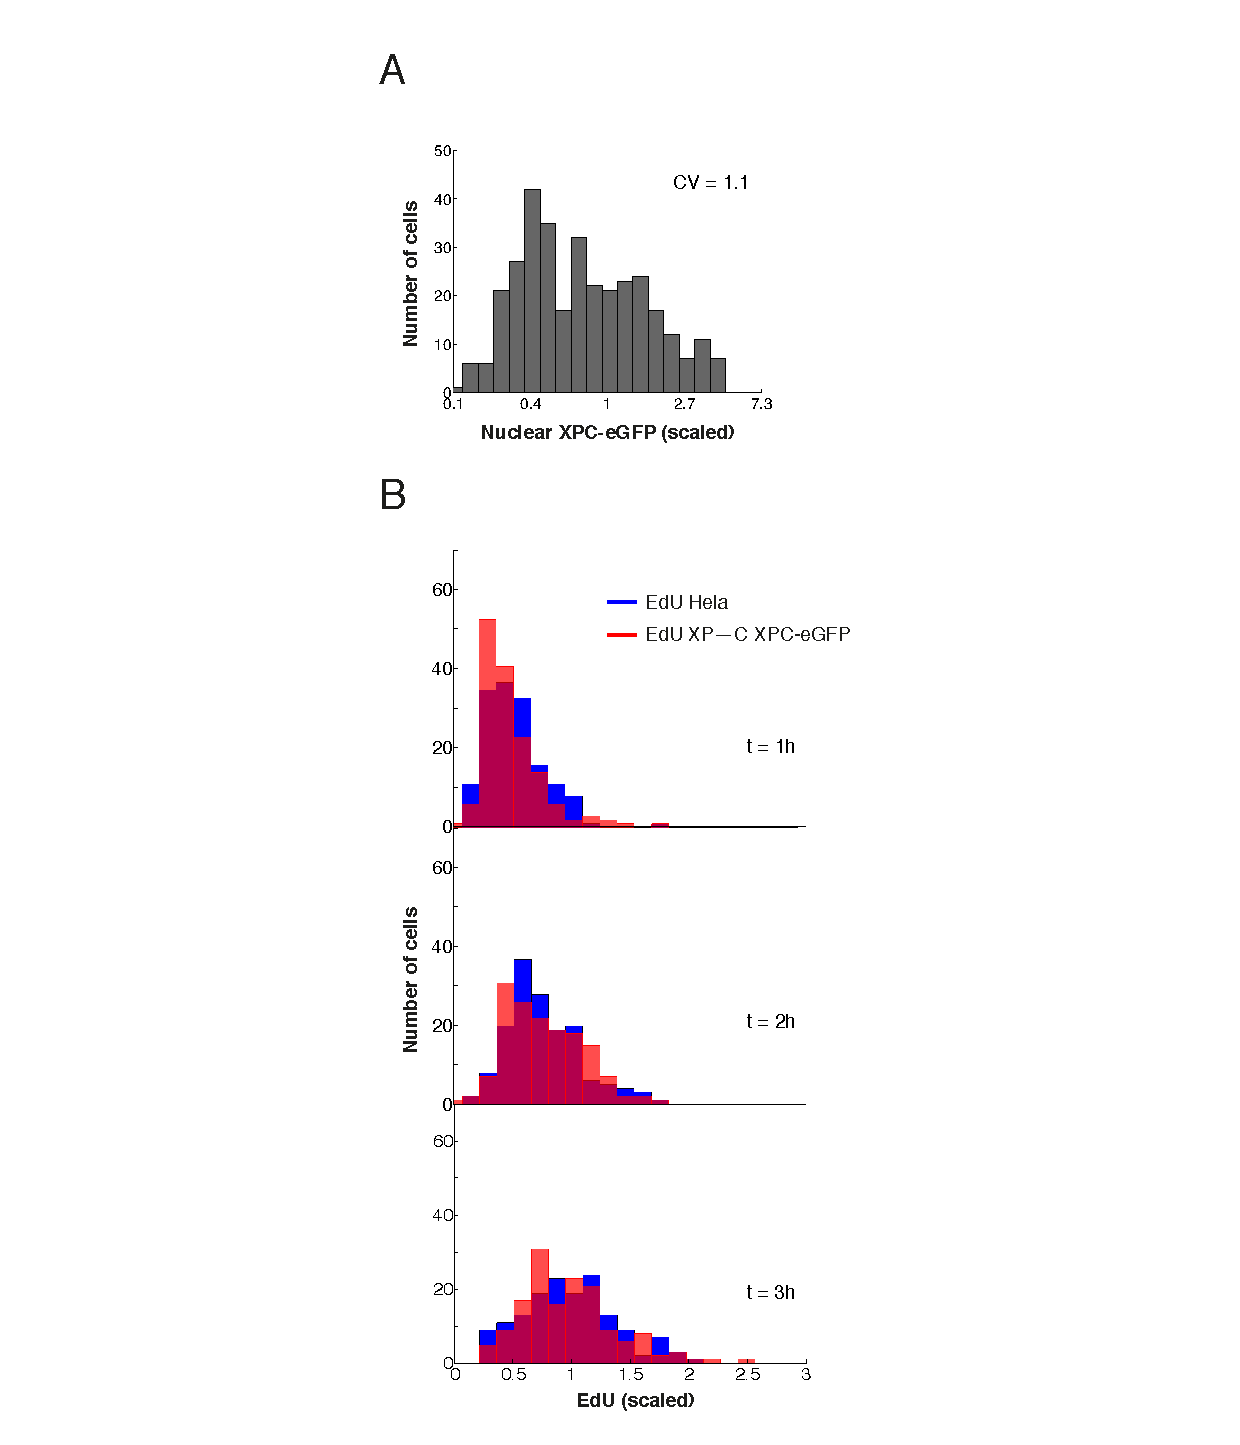
\includegraphics[width=1\textwidth]{Abbildungen/figure3_4.pdf}
		\caption{\textbf{Variability of repair synthesis is comparable between XPC-eGFP complemented XP-C patient cell lines and native NER.} A) Distribution of nuclear XPC-eGFP concentrations stably expressed in XP-C cells (n=332). B) Comparison of incorporated EdU in local damages in Hela cells (blue) and XPC-eGFP complemented XP-C cells after 1, 2 and hours (n=154 cells per time point per cell line). }
		\label{fig:consistVariability}
	\end{center}
\end{figure}

While searching for additional factors affecting the repair rate response we noticed the broad scatter of incorporated EdU, which appears to increase for larger protein concentrations (cf.\ Figure \ref{fig:Nuc_vs_DNAsynthesis}B-F). This variability indicates that, besides the repair proteins, there might be further sources of cell-to-cell heterogeneity, which might be also involved in the regulation of the repair rate. To this end, we measured the amount of UV-inflicted DNA lesions by indirect (immuno)cytochemistry to determine how the distribution of pore sizes would propagate (cf.\ Figure \ref{fig:accuMethod}B). The distributions of DNA damage captured immediately after UV-irradiation very much resembles the variable EdU incorporation after 4 hours, which is also confirmed by the similar CV. These data suggest that the amount of DNA lesions contributes to the cell-to cell variability in the repair-rate.  


\begin{figure}[htbp]
	\begin{center}
		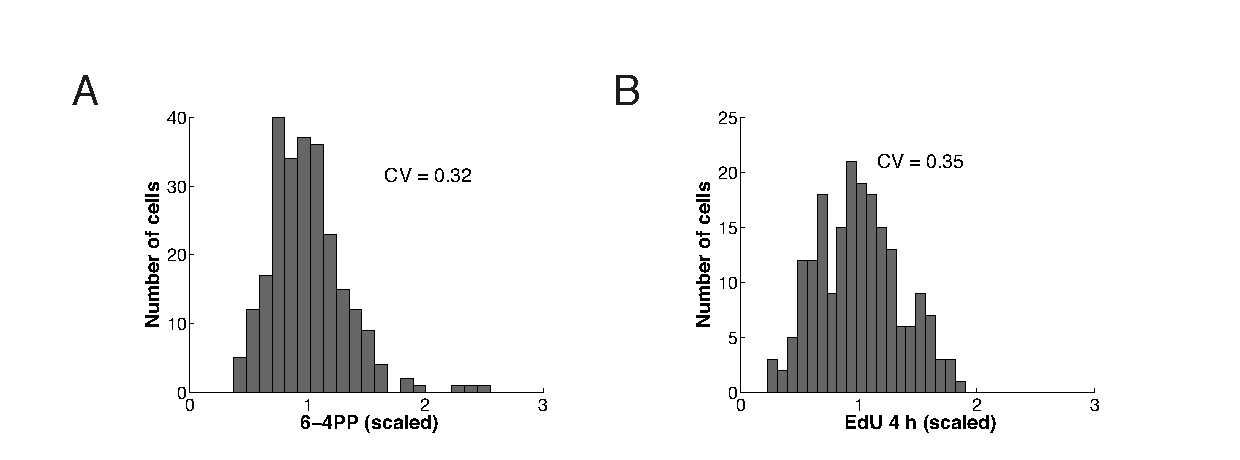
\includegraphics[width=1\textwidth]{Abbildungen/figure3_5.pdf}
		\caption{\textbf{Distributed amount of inflicted DNA damages contributes to repair rate variability.} A) XP-C XPC-eGFP cells were locally UV-irradiated with an intensity of 100 J/$\text{m}^\text{2}$. DNA damages were quantified by indirect immunofluorescence microscopy in n=250 cells from five experiments. B) XP-C XPC-eGFP cells were locally irradiated and cultivated for 4 hours in the presence of EdU before fixation. Fluorescence signals were measured in n=198 cells derived from three independent experiments. }
		\label{fig:DamageDist}
	\end{center}
\end{figure}

\begin{figure}[htbp]
	\begin{center}
		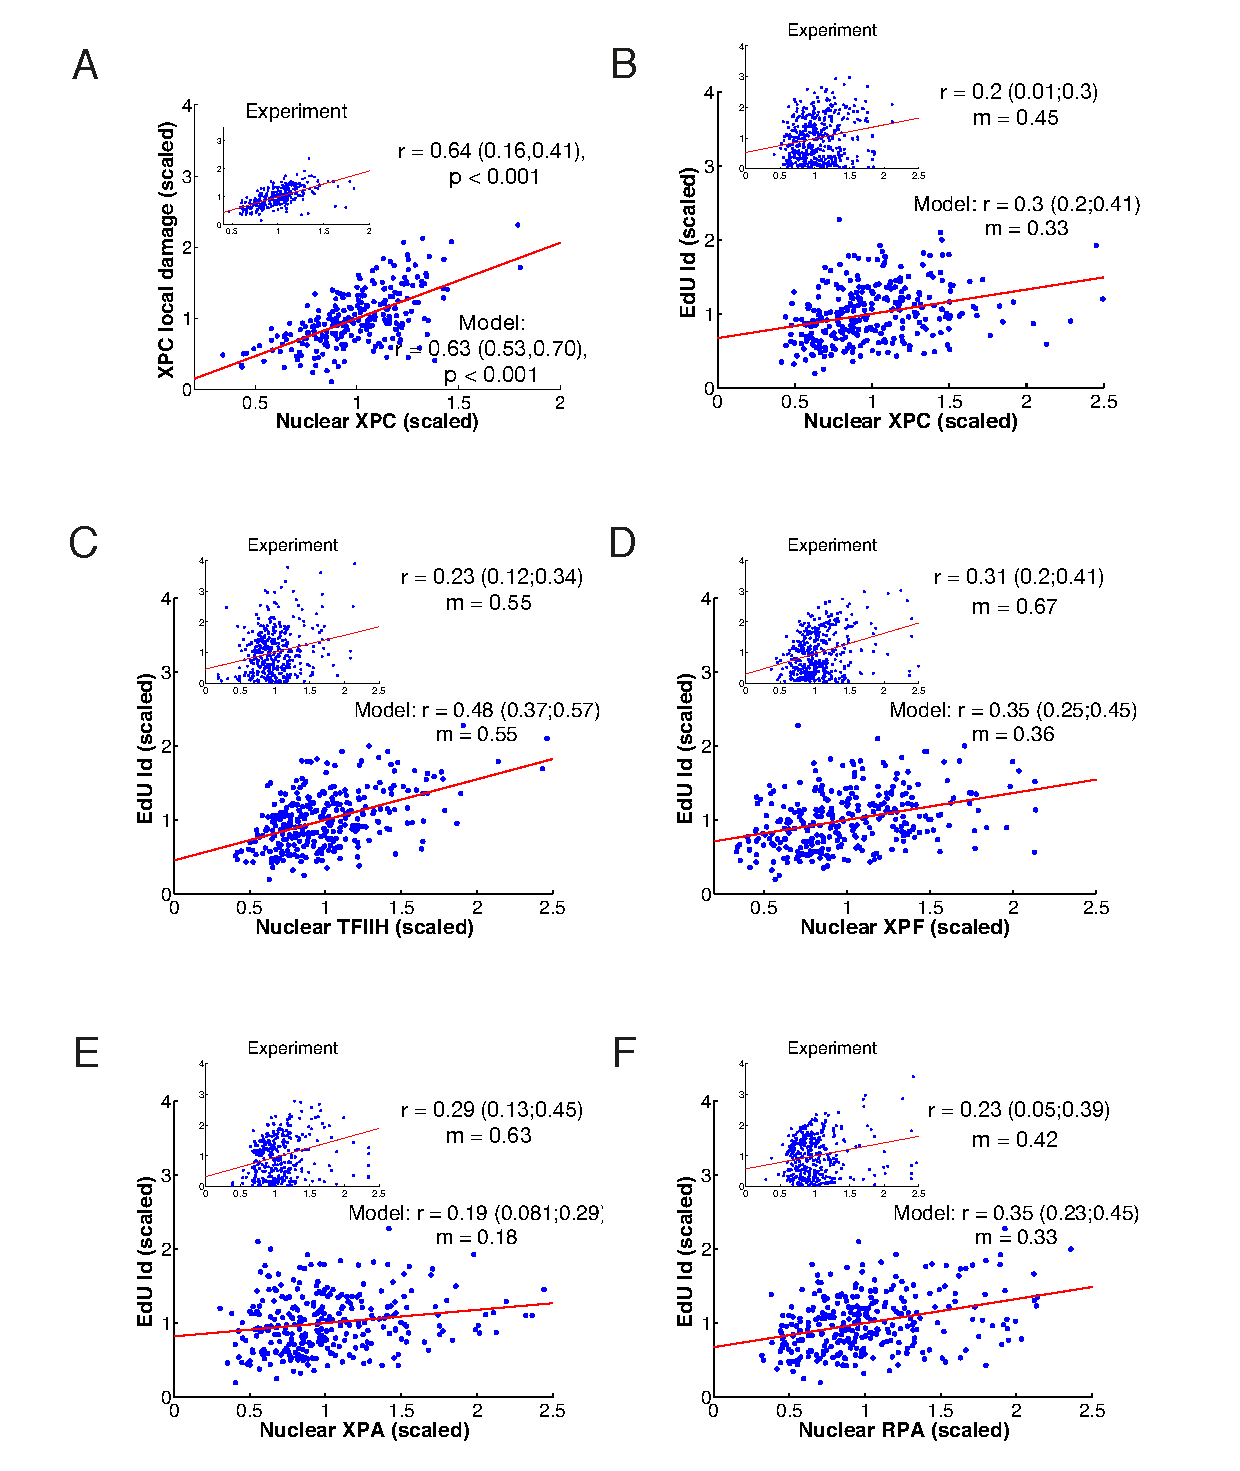
\includegraphics[width=1\textwidth]{Abbildungen/figure3_6.pdf}
		\caption{\textbf{Quantitative comparison between measured and simulated repair synthesis in response to variable NER factor concentrations.} A) Simulated scatter plot of the of locally accumulated XPC against the nuclear XPC concentration. For comparison the experimentally measured scatter plot is given in reduced size.  B-F) Comparison between measured (scatter plot in reduced size) and simulated correlation of DNA synthesis and nuclear XPC concentration. A-F) Red lines represent linear regression with correlation coefficient r, p-value and slope m. 95\% confidence bounds of all correlation coefficients r were estimated by non-parametric bootstrap and are given in brackets.}
		\label{fig:Model_dataComp}
	\end{center}
\end{figure}

To find out whether the heterogeneity in nuclear NER factor expression, together with the distributed amount of initial DNA damages, would be sufficient to explain the variability in the repair rate we tried to reproduce the EdU response measurements with the evolved quantitative model introduced in Chapter \ref{chap:kineticNERmodel}. Thus, we simulated the model several hundred times in correspondence with the number of measured cells. For each simulated cell nuclear NER factor concentrations and the amount of local damages were randomly drawn from log-normal distributions in accordance with the experimentally determined CV (cf.\ Figure \ref{fig:ProteinDist} and Figure \ref{fig:DamageDist}) and the previously measured mean values \cite{Luijsterburg2010}. For PCNA and XPG we took the averaged CV$\sim$0.33 derived from the measured distributions. \\
For XPC the simulated scatter plot for the accumulation of the nuclear repair factor at sites of local damage agree remarkably well with the measured data (cf.\ Figure \ref{fig:Model_dataComp}A, compare enlarged correlation (simulation) with the smaller inlay (experiment)). Qualitatively, the same holds true for the comparison between simulated and measured EdU incorporation as a readout for DNA resynthesis in response to changes in the repair factor concentration (cf.\ Figure \ref{fig:Model_dataComp}B-F). It should be noted that the simulated slopes representing the overall repair rate response are slightly elevated compared to the calculated response coefficients (cf.\ Figure \ref{fig:controlCoefficients}), clearly marking the influence of the introduced distribution of DNA damages. However, the simulated slopes are still significantly smaller than the measured estimates (cf.\ Figure \ref{fig:Model_dataComp}B-F, compare enlarged correlation (simulation) with the smaller inlay (experiment)). This indicates that we still miss out on an essential, perhaps intrinsic, factor regulating the repair-rate response.\\    
To locate the lacking control, we first asked whether the natural variability, contributed by the NER factor expression variability and the distribution of inflicted lesions, can explain the distribution of the repair rate. Assuming that the repair rate $\nu$ is linearly dependent on the initial amount of inflicted lesions L and, as estimated in Section \ref{firstOrderRateKinetic}, also on the nuclear repair-factor concentrations $C_i$ (i=1,2,...), we can apply the general law of error propagation
%and hence 'sums up' according to the response coefficients predicted by the model

\begin{equation}
\sigma(\nu) = \sqrt{\sum_{i}\left(\frac{\partial \nu}{\partial C_i}\sigma(C_i) \right)^2 + \left(\frac{\partial \nu}{\partial L}\sigma(L)\right)^2 }.
\label{eqn:lawoferrorPropagation}
\end{equation} 
Introducing the predicted response coefficients $R_i$ we can estimate the overall repair rate variability $CV_{\nu}$ with
\begin{equation}
CV_{\nu} = \sqrt{CV_{L}^2 + \sum_{i}(R_iCV_i)^2},
\label{eqn:lawOfErrorPropI}
\end{equation}
where $CV_{L}$ and $CV_i$ denote the coefficients of variation of the distributions of repair factors and initial amount of lesions. Obviously, the response coefficient for the initial amount of inflicted lesions is 1. Including the variability for inflicted lesions $CV_L \sim 0.32$ and the average $CV_i \sim 0.33$ for each repair factor, we can determine the repair rate variability with $CV_{\nu} \sim 0.35$. This is around 20\% less than the measured $CV_{\nu} \sim 0.45$ after one hour (cf.\ Figure \ref{fig:CV_Var_comp}).\\
\begin{figure}[b!]
	\begin{center}
		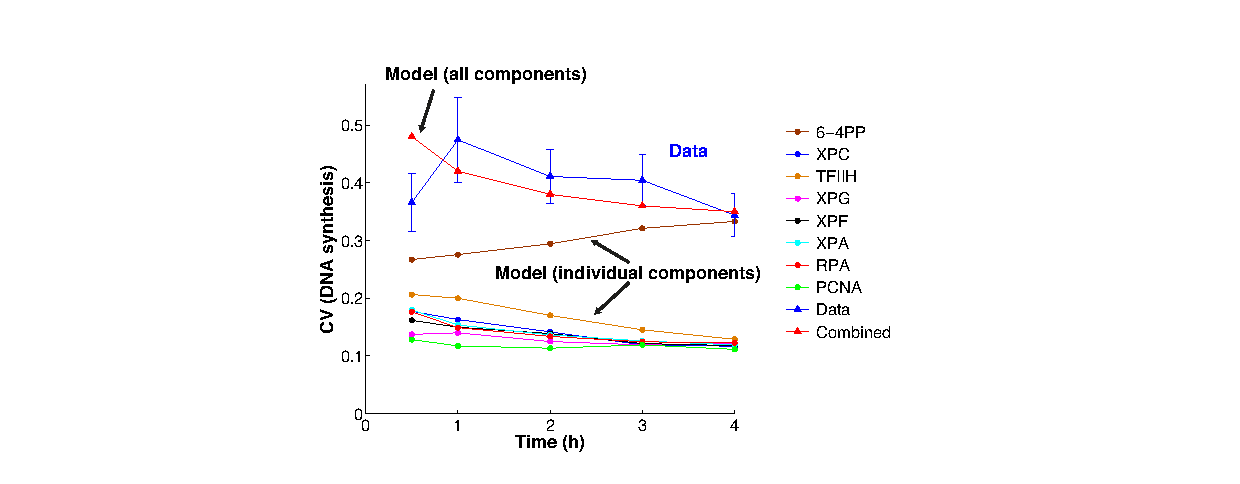
\includegraphics[width=1\textwidth]{Abbildungen/figure3_8.pdf}
		\caption{\textbf{Variability in repair synthesis results from the aggregate of initial damage variability and concentration fluctuations of each NER factor.} Each time course represents the variability in repair synthesis produced by a single component (dots) or by all components together (triangles) at a given time. For comparison the experimental measured distribution of incorporated EdU is shown in blue. Error bars depict the 95\% confidence intervals determined with non-parametric bootstrap.}
		\label{fig:CV_Var_comp}
	\end{center}
\end{figure}
\noindent To dissect the contribution of the individual factors to the
overall variability, we computed the effect of heterogeneity in only one factor on repair synthesis. Accordingly, for each CV-trajectory in Figure \ref{fig:CV_Var_comp} we determined the $CV_{\nu}$ by simulating the repair rate for 500 cells and drawing only one factor randomly. The largest contribution can be allocated to the initial amount of damages (cf.\ Figure \ref{fig:CV_Var_comp} brown trajectory) which were responsible for about two thirds of the whole repair variability (cf.\ Figure \ref{fig:CV_Var_comp} blue trajectory). Drawing all NER factors together with the initial amount of damages from their pre-determined distributions shrinks the gap between measured and simulated DNA repair variability (cf.\ Figure \ref{fig:CV_Var_comp} blue (data) and red (simulation) trajectory).\\
This result becomes more explicit, as seen, by comparing the strikingly matching temporal evolution of the measured and predicted distributions of repair synthesis (cf.\ Figure \ref{fig:ModelData_tempVar}).\\




To summarize, in this chapter we uncovered two sources of natural variability that are propagated throughout the repair process and consequently contributing to the emergent cell-to-cell variability of repair synthesis: (i) the amount of inflicted DNA lesions and (ii) the variation of the nuclear NER factor concentrations. 
However, the significant differences between measured and predicted repair rate responses (cf.\ Figure \ref{fig:Model_dataComp}, compare the slope $m$ of the regression lines) leave space for interpretation, whether there are additional factors involved in repair, but have not been accounted for, explicitly, in the model.

\begin{figure}[htbp]
	\begin{center}
		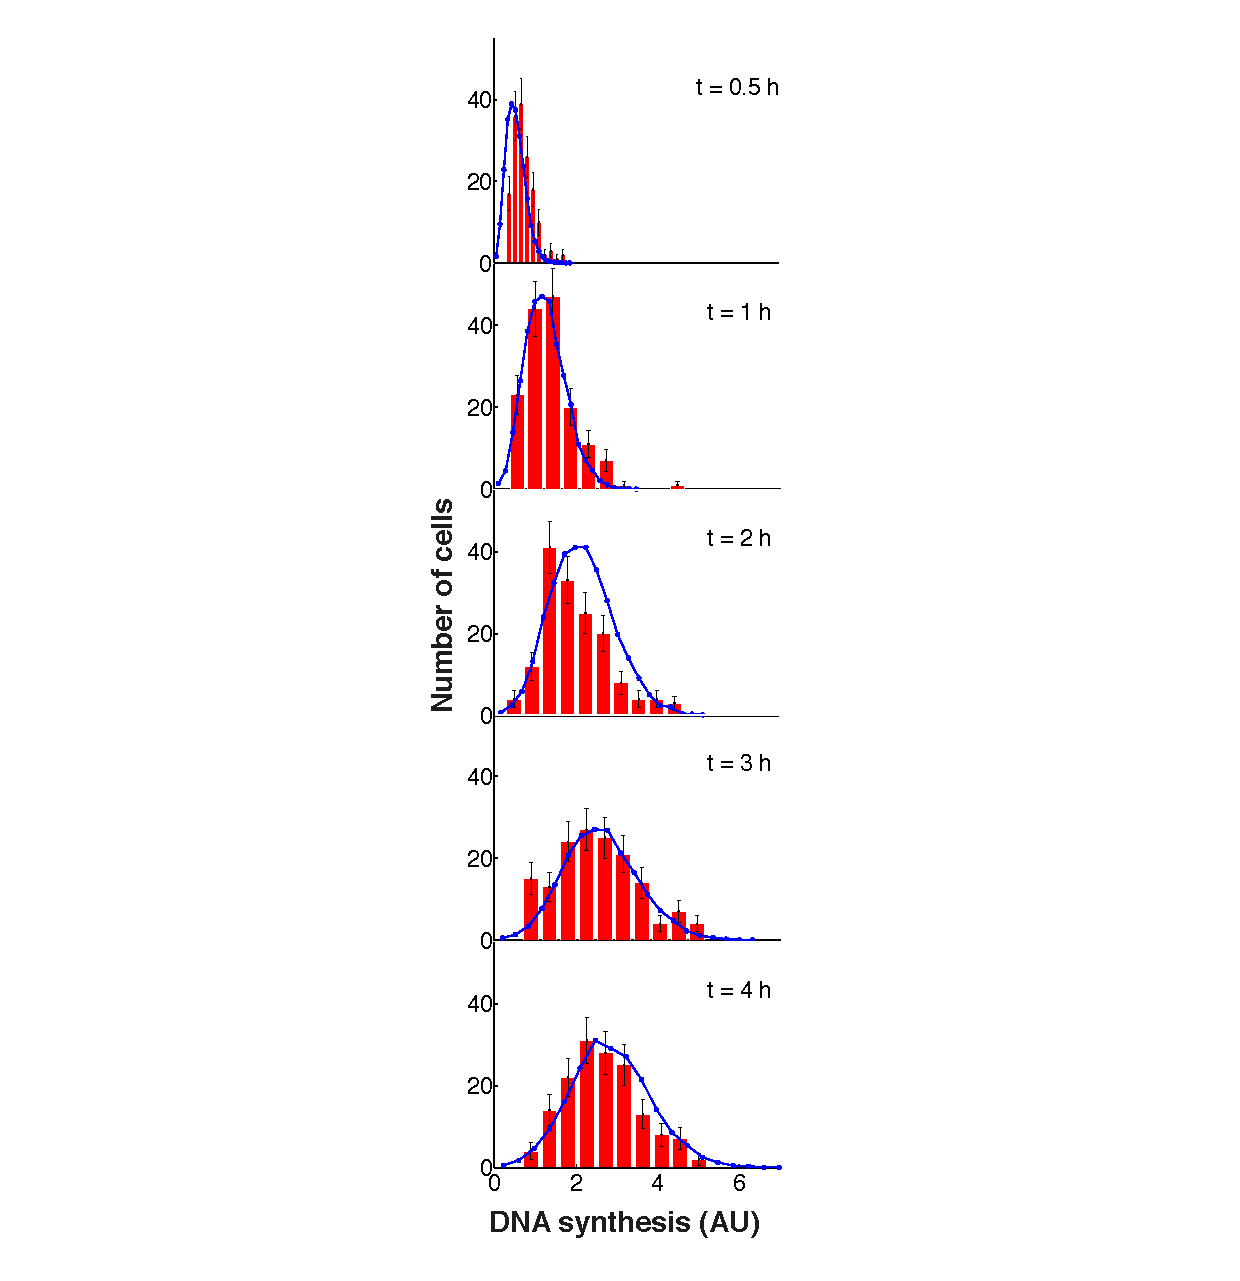
\includegraphics[width=1\textwidth]{Abbildungen/figure3_7.pdf}
		\caption{\textbf{Simulated repair rate distribution fits experimentally derived EdU incorporation} Temporal evolution of the repair rate variation i)  measured in single cells after initial UV-irradiation (red histograms) and ii) predicted from model simulations (blues lines).}
		\label{fig:ModelData_tempVar}
	\end{center}
\end{figure}